
%
\item From the given info, 
    \begin{align}
    \vec{x}^T \myvec{3 & 0\\0 & 0}\vec{x}+ 2\myvec{\frac{-5}{2} \\ \frac{-1}{2}}\vec{x}+2=0
\end{align}
    \begin{align}
    \implies     \vec{V} = \myvec{3 & 0 \\ 0 & 0},\vec{u}=\myvec{\frac{-5}{2} \\ \frac{-1}{2}},f=2
    \end{align}
     Using eigenvalue decomposition,
    \begin{align}
        \vec{D} = \myvec{0 & 0\\0 & 3} ,\vec{P}=\myvec{0 & 1\\1 & 0}
    \end{align}
Also, 
\begin{align}
    \myvec{\vec{u}^T + \eta\vec{p_1}^T \\ \vec{V}}\vec{c} &= \myvec{-f \\ \eta\vec{p_1}-\vec{u}} 
\end{align}
%
    \begin{align}
\implies         \myvec{\frac{-5}{2} & -1 \\ 3 & 0 \\ 0 & 0}\vec{c} &= \myvec{-2 \\ \frac{5}{2} \\ 0} \\
     \implies  \myvec{\frac{-5}{2} & -1 \\ 3 & 0}\vec{c} &= \myvec{-2 \\ \frac{5}{2}}
        \\
        \implies \vec{c} &= \myvec{\frac{5}{6}\\\frac{-1}{12}}
    \end{align}
    $\because $
    \begin{align}
        \vec{p_1}^T\vec{c} &= \myvec{0 & 1}\myvec{\frac{5}{6}\\\frac{-1}{12}}
        \\
        &= \frac{-1}{12}
    \end{align}
    and,
    \begin{align}
        \vec{p_2}^T\vec{V}\vec{p_2} &= \myvec{1 & 0}\myvec{3 & 0\\0& 0}\myvec{1 \\ 0}
        \\
        &= 3
    \end{align}
    %
    \begin{align}
    (\vec{p_1}^T\vec{c})(\vec{p_2}^T\vec{V}\vec{p_2}) = \frac{-1}{4}<0
    \end{align}
    Hence,the given equation has real roots which is verified in Fig.  \ref{quad/2/23/ex3}.	
        %
        \begin{figure}[!ht]
            \centering
            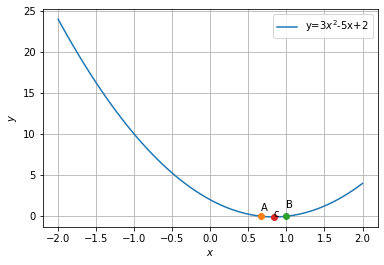
\includegraphics[width=\columnwidth]{solutions/su2021/2/23/figure5(1).png}
            \caption{$y=3x^2-5x+2$}
            \label{quad/2/23/ex3}	
            \end{figure}
        
 \item
    \begin{align}
        y &= x^2+4x+5
    \end{align}
    Here,
    \begin{align}
        \vec{V} = \myvec{1 & 0 \\ 0 & 0},\vec{u}=\myvec{2 \\ \frac{-1}{2}},f=5
    \end{align}
    %
    Using eigenvalue decomposition,
    \begin{align}
        \vec{D} = \myvec{0 & 0\\0 & 1} ,\vec{P}=\myvec{0 & 1\\1 & 0}
    \end{align}
    Now,
\begin{align}
    \myvec{\vec{u}^T + \eta\vec{p_1}^T \\ \vec{V}}\vec{c} &= \myvec{-f \\ \eta\vec{p_1}-\vec{u}} 
\end{align}
    $\therefore$
    \begin{align}
        \myvec{2 & -1 \\ 1 & 0 \\ 0 & 0}\vec{c} &= \myvec{-5 \\ 2 \\ 0} \\
        \implies  \myvec{2 & -1 \\ 1 & 0}\vec{c} &= \myvec{-5 \\ 2}
        \\
        \implies \vec{c} &= \myvec{2\\1}
    \end{align}
    
    $\because $
    \begin{align}
        \vec{p_1}^T\vec{c} &= \myvec{0 & 1}\myvec{2 \\ 1}
        \\
        &= 1
    \end{align}
    and
    \begin{align}
        \vec{p_2}^T\vec{V}\vec{p_2} &= \myvec{1 & 0}\myvec{-1 & 0\\0& 0}\myvec{1 \\ 0}
        \\
        &= 1
    \end{align}
    %
    \begin{align}
        (\vec{p_1}^T\vec{c})(\vec{p_2}^T\vec{V}\vec{p_2}) = (1)(1) = 1>0
        \end{align}
        Hence,the given equation does not have real roots which is verified in Fig.     \ref{quad/2/23/ex4}	
    \begin{figure}[!ht]
    \centering
    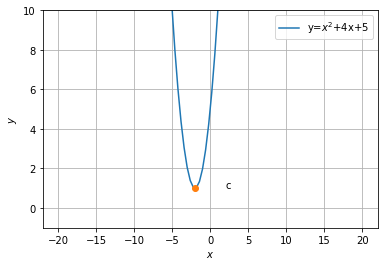
\includegraphics[width=\columnwidth]{solutions/su2021/2/23/figure5(2).png}
    \caption{$y=x^2+4x+5$}
    \label{quad/2/23/ex4}	
    \end{figure}
    
   
   
   
   